\chapter{La señal EEG y su modelo matemático}
\label{cap:senal}

\section{Origen fisiológico del EEG}

El EEG de superficie registra diferencias de potencial eléctrico entre electrodos ubicados sobre el cuero cabelludo. La señal se origina principalmente en las corrientes postsinápticas de las neuronas piramidales de la corteza, que están orientadas en paralelo: cuando grandes poblaciones se activan en sincronía, sus campos se suman y generan potenciales del orden de decenas de microvoltios.

\pendiente{1--2 páginas: sistema 10-20, montaje bipolar ``doble banana'', artefactos (parpadeo, músculo, red eléctrica).}

\section{Ritmos cerebrales}

Tradicionalmente la actividad del EEG se describe en bandas de frecuencia (tabla~\ref{tab:bandas}).

\begin{table}[ht]
\centering
\caption{Bandas clásicas del EEG usadas en este trabajo.}
\label{tab:bandas}
\begin{tabular}{@{}llp{7cm}@{}}
\toprule
Banda & Rango [Hz] & Asociación típica \\
\midrule
$\delta$ (delta) & 0,5--4 & Sueño profundo; actividad lenta patológica \\
$\theta$ (theta) & 4--8 & Somnolencia; frecuente en el inicio de crisis \\
$\alpha$ (alfa) & 8--13 & Vigilia relajada con ojos cerrados \\
$\beta$ (beta) & 13--30 & Actividad cognitiva, vigilia activa \\
$\gamma$ (gamma) & 30--45 & Procesamiento local; también artefacto muscular \\
\bottomrule
\end{tabular}
\end{table}

\section{Modelo matemático de la señal}

Se modela el EEG de un canal como una suma de oscilaciones en las bandas de la tabla~\ref{tab:bandas} más un fondo aperiódico:
\begin{equation}
x(t) = \sum_{b \in \{\delta,\theta,\alpha,\beta,\gamma\}} A_b(t)\,\sin\!\big(2\pi f_b(t)\,t + \varphi_b(t)\big) + \eta(t),
\qquad S_\eta(f) \propto \frac{1}{f^{\beta}},
\label{eq:modelo_eeg}
\end{equation}
donde $A_b(t)$ y $f_b(t)$ varían lentamente respecto del período de cada oscilación y $\eta(t)$ es un proceso aleatorio cuya densidad espectral decae como una ley de potencia (ruido ``$1/f$''), con $\beta$ típicamente entre 1 y 2.

En reposo la potencia se reparte entre varias bandas y el fondo $1/f$ tiene un peso importante. Durante una crisis, una población grande de neuronas se \emph{hipersincroniza}. En el modelo~\eqref{eq:modelo_eeg} esto se traduce en:
\begin{enumerate}
  \item un término dominante $A_{b^\star}(t) \gg A_b(t)$ para $b \neq b^\star$, con $f_{b^\star}$ típicamente entre 3 y 8~Hz y a menudo con armónicos;
  \item la aparición del mismo ritmo, con fases relacionadas, en varios canales (aumento de la \emph{coherencia});
  \item un aumento de la amplitud total y de la variación de la señal en el tiempo (\emph{line length}).
\end{enumerate}

La consecuencia espectral central es que la potencia se \emph{concentra} en pocas frecuencias. El capítulo~\ref{cap:fourier} cuantifica esta concentración con la entropía espectral y demuestra que su valor máximo corresponde a una señal sin estructura (ruido blanco).

\section{La base de datos CHB-MIT}

\pendiente{describir sujetos, edades, registros, anotaciones; incluir figura \texttt{datos\_crisis} y \texttt{eeg\_crisis\_multicanal} del notebook (sección 1 y 2).}

\begin{figure}[ht]
\centering
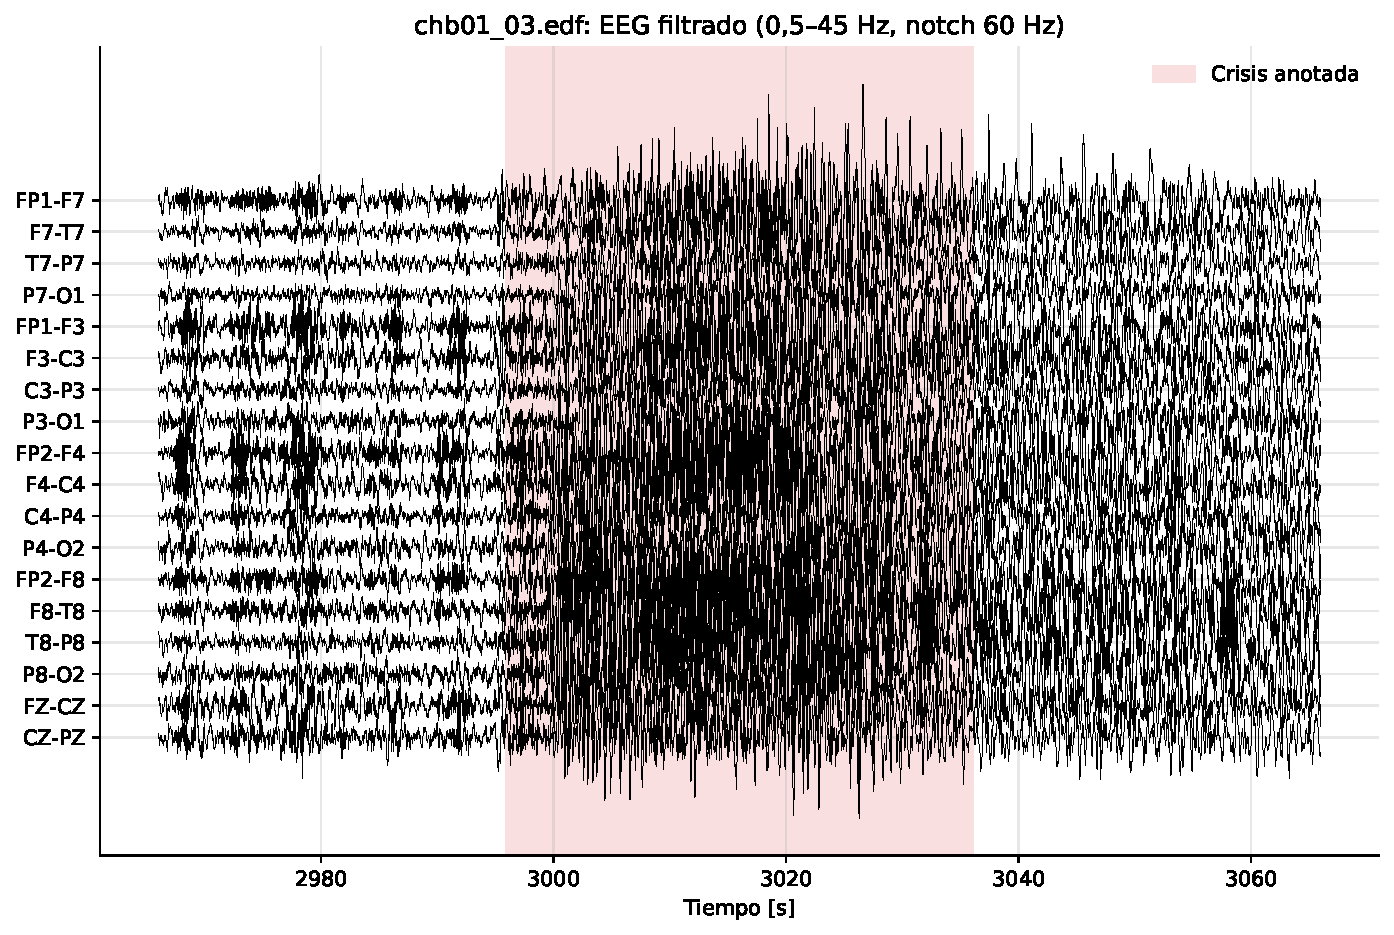
\includegraphics[width=\linewidth]{eeg_crisis_multicanal}
\caption{EEG filtrado de los 18 canales bipolares alrededor de una crisis anotada (sombreado).}
\label{fig:eeg_crisis}
\end{figure}
